\chapter{Bejelentkezés}

\begin{itemize}
    \item Szükséges megadni az alábbi adatokat a bejelentkezéshez:
    \begin{itemize}
        \item \textbf{Email cím}
        \item \textbf{Jelszó}
    \end{itemize}
\end{itemize}
\begin{minipage}[h]{0.5\textwidth}
    \begin{center}
        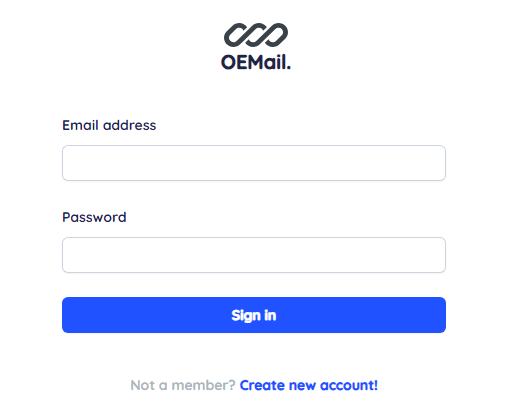
\includegraphics[width=1\textwidth]{login}
    \end{center}
\end{minipage}%
\begin{minipage}[h]{0.5\textwidth}
    \begin{center}
        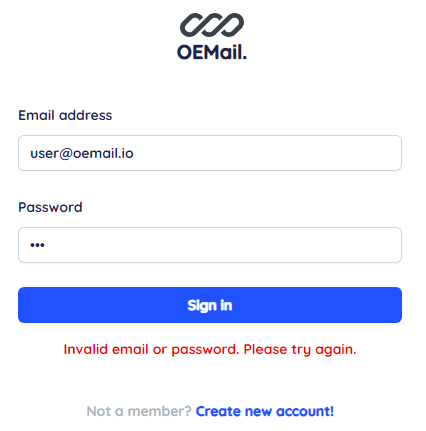
\includegraphics[width=0.9\textwidth]{failed_login}
    \end{center}
\end{minipage}%
\begin{flushleft}
    Bejelentkezés után automatikus a felhasználó át lesz irányítva a \verb|http://localhost:5173/mail| főoldalra. A bal oldali sávban tud a felhasználó navigálni az oldalon, ahol az alábbi menüpontok találhatóak meg:
    \begin{minipage}[h]{0.5\textwidth}
        \begin{itemize}
            \item Főoldal (Home)
            \item Új üzenet küldése (Send new message)
            \item Beérkezett üzenetek (Inbox)
            \item Elküldött üzenetek (Sent)
            \item Szemét (Trash)
            \item Csillagozott (Starred)
            \item Gyanús üzenetek (Spam)
        \end{itemize}
    \end{minipage}%
    \begin{minipage}[h]{0.5\textwidth}
        \begin{center}
            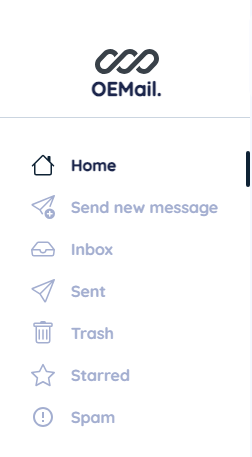
\includegraphics[width=0.7\textwidth]{nav}
        \end{center}
    \end{minipage}%
    
\end{flushleft}